%**************************************************************************************
\section{Phenomenology and Modeling of Bottom Reflood}\label{sec:reflood_phenomenology}
%**************************************************************************************

% Opening Paragraph, the reflood phase
As mentioned in the opening of this chapter, reflood phase is the last phase of the four canonical phases in the mitigation of \gls[hyper=false]{lbloca} in \glspl[hyper=false]{lwr},
\marginpar{Reflood phase in LBLOCA}
in which emergency coolant water flows slowly upward through the reactor core, quenching the fuel elements along the way.
The phase is expected to occur after the refill phase, in which a successful injection of the water through the downcomer and lower plenum of the \gls[hyper=false]{rpv}.

% Reflooding
\emph{Quenching} (or \emph{rewetting}) refers to the phenomenon in which a sustainable contact between the liquid phase of the coolant and the hot surfaces of the fuel is re-established.
\marginpar{Quenching}
Prior to the quenching, the excessively high surface temperature prevents a stable contact between the liquid phase and the surface, degrading the heat transfer between the two.
The maximum temperature for which the liquid might make a stable contact with the surface is referred to as the \emph{quenching temperature}.
In consequence, although the bulk of the flow through the core is liquid, the inability for the liquid to make contact with the surface keeps it at a very high temperature \cite{Hewitt2000,Zeng2010}.

In \gls[hyper=false]{bwr}, reflood might also occurs by spraying the core from the top resulting in the \emph{top reflood};
\marginpar{Top and bottom reflood}
while in both \gls[hyper=false]{bwr} and \gls[hyper=false]{pwr}, injection of water downward through the downcomer and upward through the core is termed \emph{bottom reflood}.
There are different physical processes associated with the two, such as the fact that in the top reflood there is steam flow from the bottom of the channel pushing back the liquid injection.
This thesis is only concerned with the bottom reflood. 
As the process sets a limiting ability for the emergency coolant to bring about efficient cooling to the fuel elements in the \gls[hyper=false]{lbloca} transient, a proper modeling of the physical processes associated with the reflood phase is an important for the safety analysis of \glspl[hyper=false]{lwr}.

% Reflood curve
A typical mid-height cladding temperature evolution in a channel undergoing a bottom reflood 
\marginpar{Reflood curve}
(so-called \emph{reflood curve}) can be seen in Fig.~\ref{fig:ch2_reflood_curve_qois} under a constant coolant injection rate and a constant power boundary condition.
\begin{figure}[bth]
    \centering
    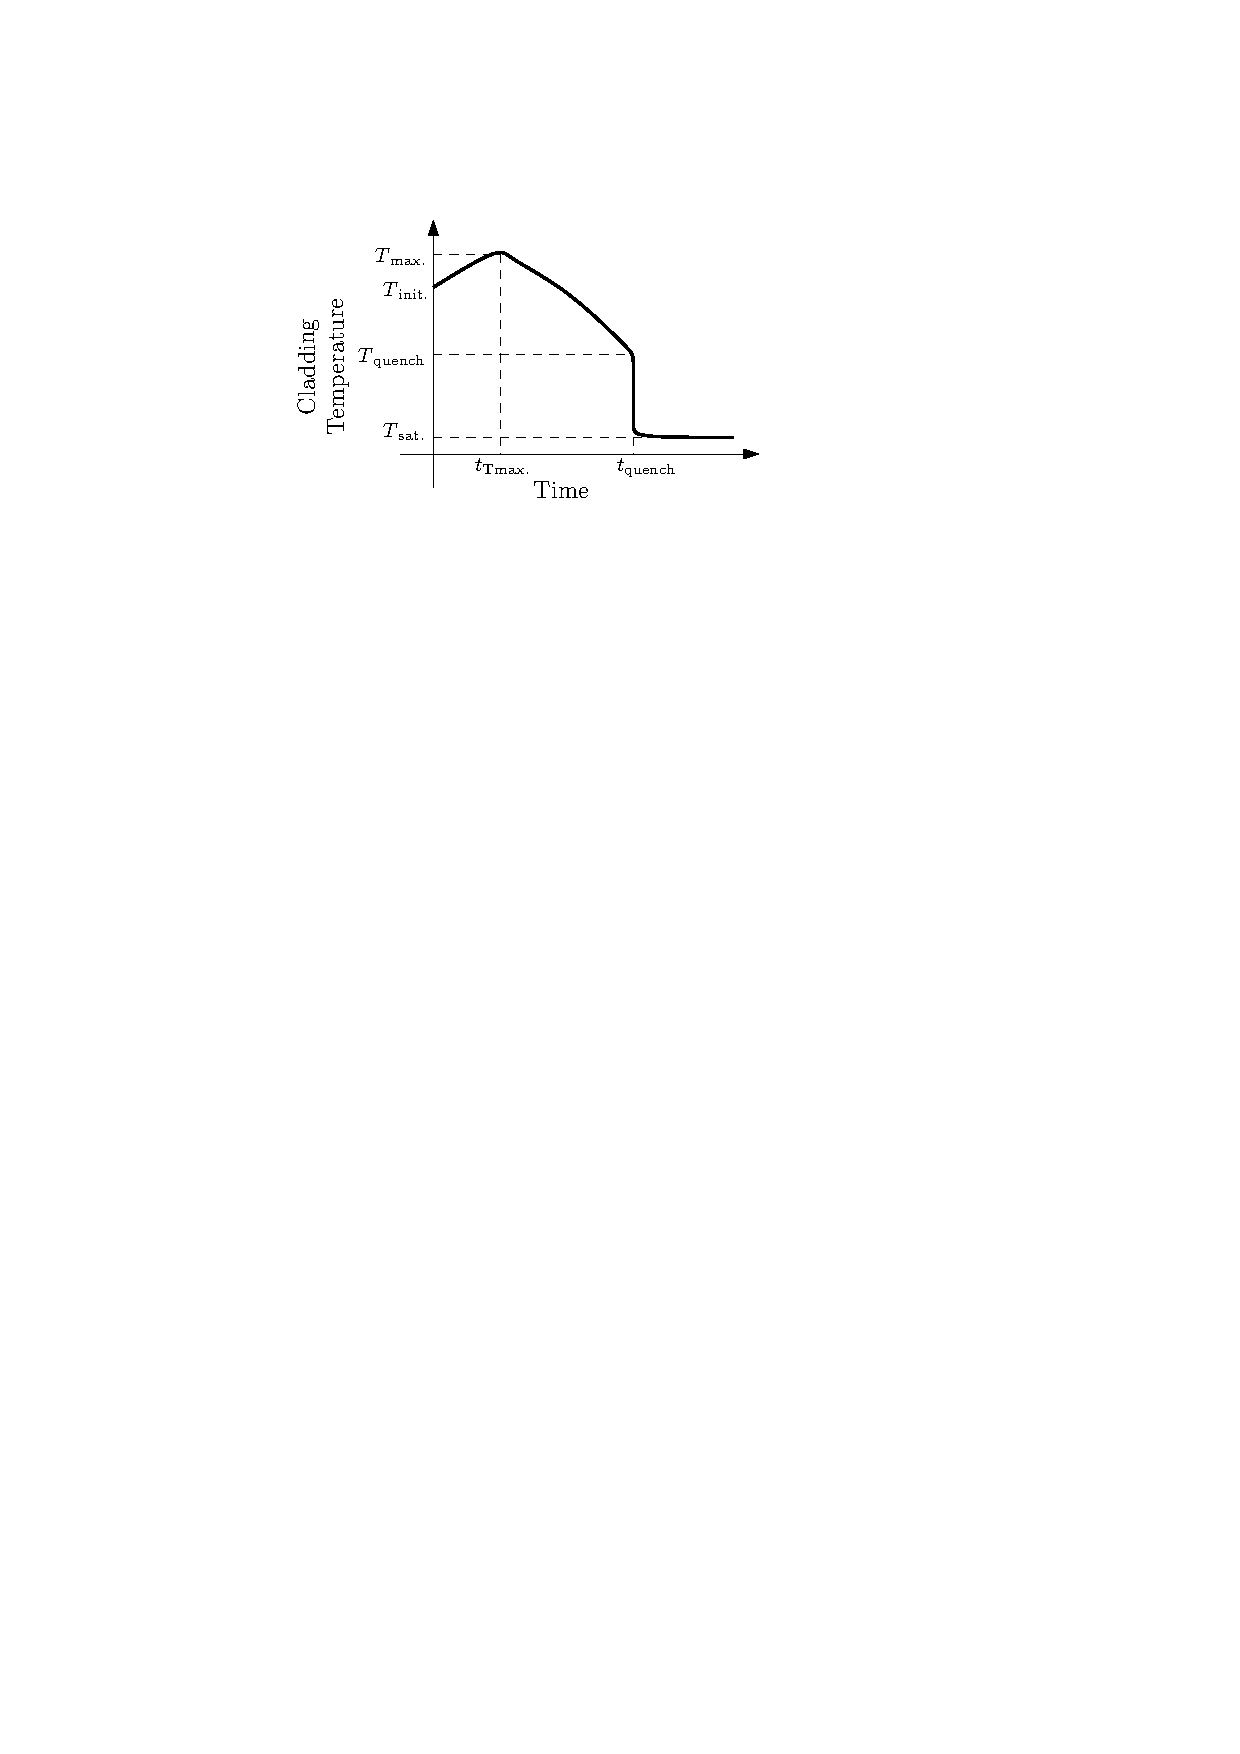
\includegraphics[width=1.0\textwidth]{../figures/chapter2/figures/refloodCurveQoIs}
    \caption[A typical cladding temperature evolution during constant flooding rate reflooding at mid-height assembly.]{A typical cladding temperature evolution during constant flooding rate reflooding at mid-height assembly (adapted from \cite{Zeng2010}). The labels on the both axes are typical \glspl[hyper=false]{qoi} of reflood transient, where the abbreviations $max.$, $init.$, and $sat.$ refer to the \emph{maximum}, \emph{initial}, and \emph{saturation}, respectively.}
    \label{fig:ch2_reflood_curve_qois}
\end{figure}

At the start of the transient (cladding temperature at $T_\text{init.}$) the channel consists purely of steam.
Keeping the power constant increases the cladding temperature up until mixture of steam and liquid (droplets) arrives at the location, improving the heat transfer mechanism, and decreasing the temperature ($T_\text{max.}$ at $t_{T_\text{max.}}$).
As the channel keeps undergoing reflood from the bottom, more droplets are available at the location to keep decreasing the cladding temperature.
Moreover, as the quenching happens below this particular location, large axial temperature gradient in the cladding is present and is further accelerating the heat conduction from the un-quenched part to the quenched part of the cladding.
Finally, when the temperature of the cladding reaches the quenching temperature ($T_\text{quench}$ at $t_{\text{quench}}$)), quenching occurs and stable contact between liquid and the cladding can be established.
From that point onward, the cladding temperature is in equilibrium with the liquid at saturation.

% The Modeling of The Phenomenology
The phenomenological view of the process, adopted by \gls[hyper=false]{trace} code \cite{USNRC2012}, is shown in Fig.~\ref{fig:ch2_post_chf_regime} along with the corresponding part in the reflood curve of Fig.~\ref{fig:ch2_reflood_curve}.
\marginpar{Reflood, phenomenology}
The post-\gls[hyper=false]{chf} flow regimes (regimes $(2)$--$(5)$ in the figure) are in-between two pre-\gls[hyper=false]{chf} flow regimes, namely nucleate boiling at the bottom and steam convection at the top.
\normdoublefigure[pos=!h,
                  mainlabel={fig:ch2_reflood_phenomenology},
                  maincaption={Phenomenology of flow during reflood according to \gls[hyper=false]{trace} code and the corresponding part of the transient in the reflood curve.},
				mainshortcaption={Phenomenology of flow during reflood according to \gls[hyper=false]{trace} code.},
                  leftopt={width=0.45\textwidth},
                  leftlabel={fig:ch2_post_chf_regime},
                  leftcaption={post-\gls[hyper=false]{chf} flow regimes $(2)$--$(5)$},
                  %leftshortcaption={},%
                  rightopt={width=0.5\textwidth},
                  rightlabel={fig:ch2_reflood_curve},
                  rightcaption={Reflood curve}]
{../figures/chapter2/figures/postCHFRegime}
{../figures/chapter2/figures/refloodCurvePhenomenology}

% Steam Flow
Consider a case of injecting subcooled liquid water with a constant feed rate (i.e., \emph{flooding rate}) into a dry heated channel.
At the given location of the temperature probe at the start of the transient, steam convection (regime~($2$) in Fig.~\ref{fig:ch2_post_chf_regime}) is the dominant heat transfer mechanism and the cladding temperature keeps increasing.
In \gls[hyper=false]{trace}, the steam convection process belongs to the pre-\gls[hyper=false]{chf} package \cite{USNRC2012}.

% DFFB
As the bottom part of the channel is quenched (the point of quenching on the surface is referred to as \emph{quench front}) three flow regimes can be observed.
\marginpar{\Glsfirst[hyper=false]{dffb}}
Far from the quench front, liquid droplets are dispersed and carried away by the bulk steam flow.
The flow regime, called \glsfirst[hyper=false]{dffb}, provides an improved heat transfer mechanism from the wall to the fluid as compared to the pure steam convection through direct radiation to the droplets, convection to the droplets and convection to the steam.
The droplets provide additional heat sink from the bulk steam flow.
The presence of the droplets in the flow also further enhance the turbulence of the steam flow improving the convection from the wall to the steam flow \cite{Zeng2010}.
The improvement to heat transfer brought by these mechanisms allows the cladding temperature to reach a maximum and decrease.

% Inverted Slug
As the quench front progresses upward, not too far from the front a more efficient cooling is provided from morphologically less regular entrained liquid, called ligaments or slugs (regime~($3$) in Fig.~\ref{fig:ch2_post_chf_regime}).
\marginpar{Inverted Slug}
Due to this efficient cooling, the cladding temperature keeps decreasing.
The slug flow regime is inverted in the sense that the slugs are of the liquid phase. 
In \gls[hyper=false]{trace} these slugs are modeled as prolate ellipsoids.
The flow regime itself represents an interpolatory region between the previous \glsentryshort{dffb} flow regime and the subsequent \gls[hyper=false]{iafb} flow regime \cite{USNRC2012}.

% IAFB
Closer to the front, the bulk of the subcooled liquid flow starts to appear in front of the surface.
\marginpar{\Glsfirst[hyper=false]{iafb}}
However, a thin vapor film still separates the liquid from the wall and thus prevents an ideal heat transfer to occur.
In this so-called \glsfirst[hyper=false]{iafb} flow regime (regime~($4$) in Fig.~\ref{fig:ch2_post_chf_regime}), the bulk of the coolant flow in the center of the channel is liquid (i.e., the liquid core).
The heat transfer mechanism from the wall is through convection to the vapor film and direct radiation to the liquid core \cite{Zeng2010,USNRC2012}.

% Transition Boiling
Finally, as quenching becomes imminent and the cladding temperature reaches the quenching temperature, the flow regime switch to the unstable \emph{transition boiling}, which literally means the transition between dry wall and wet wall regimes.
\marginpar{Transition boiling}
In \gls[hyper=false]{trace} the heat transfer is evaluated based on the look-up table \gls[hyper=false]{chf} at the particular flow conditions.
It results in a very large \gls[hyper=false]{htc} between the wall and the fluid and causes the rapid drop (i.e., quenching) of the temperature (regime~($5$) in Fig.~\ref{fig:ch2_post_chf_regime}). 
After quenching, the cladding surface is in full contact with the liquid.
The cladding temperature is in equilibrium with the bulk flow of saturated liquid and the flow regime involves different phenomena, namely nucleate boiling (regime~($6$) in Fig.~\ref{fig:ch2_post_chf_regime}).
In \gls[hyper=false]{trace}, as the steam convection, the nucleate boiling process belongs to the pre-\gls[hyper=false]{chf} package \cite{USNRC2012}.